\documentclass{beamer}

\usepackage[utf8]{inputenc}
\usepackage[russian]{babel}

\usepackage{amsmath}

\graphicspath{{figures/}}

\uselanguage{russian}
\languagepath{russian}
\deftranslation[to=russian]{Theorem}{Теорема}
\deftranslation[to=russian]{theorem}{теорема}


\mode<presentation>{


\usetheme{Warsaw}

\usetheme{Warsaw}

\title{Замощения плоскости и пространства}

\institute[ФТЛ]{Физтех-лицей \\ \medskip \slshape  feldman@wowmath.ru}

\author{Григорий Фельдман}

\date{12 сентября 2015}


\begin{document}

\begin{frame}
\titlepage
\end{frame}


\begin{frame}


%Замощения плоскости
%
Кто из нас не увлекался рисованием интересных орнаментов на бумаге? 

\centerline{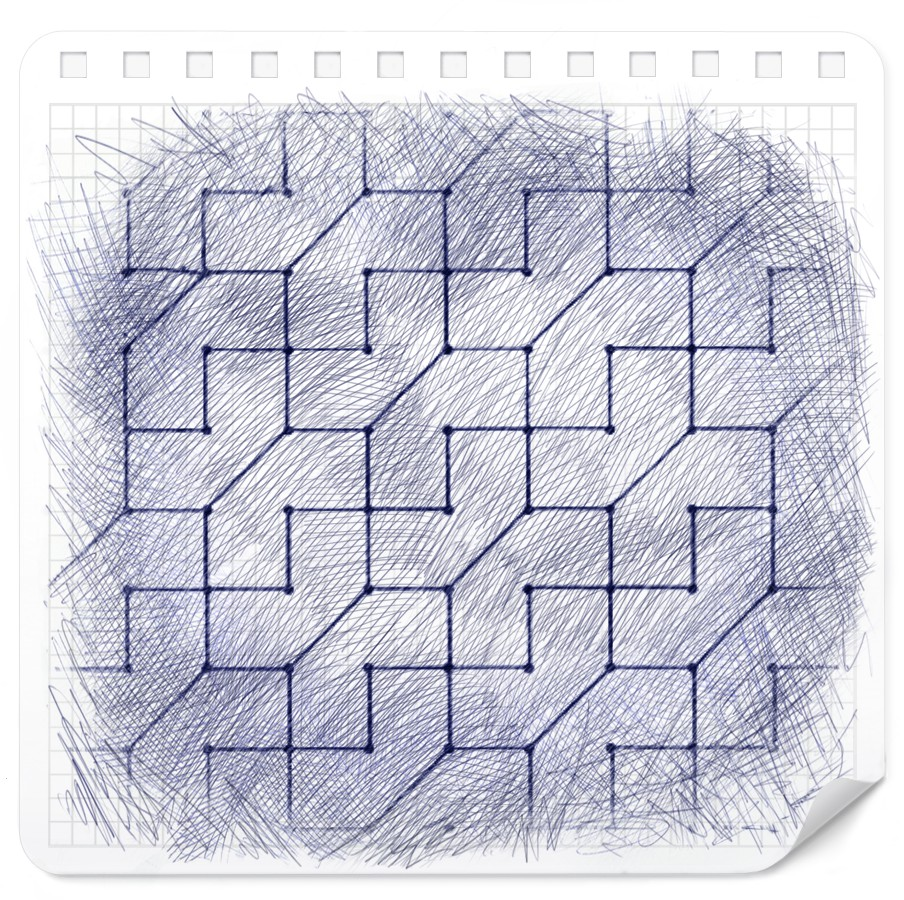
\includegraphics[width=.7\textwidth]{tess_pen.jpg}}

\end{frame}


\begin{frame}
Некоторые даже стали заниматься этим профессионально и кладут плитку на дорогах.

\begin{center}
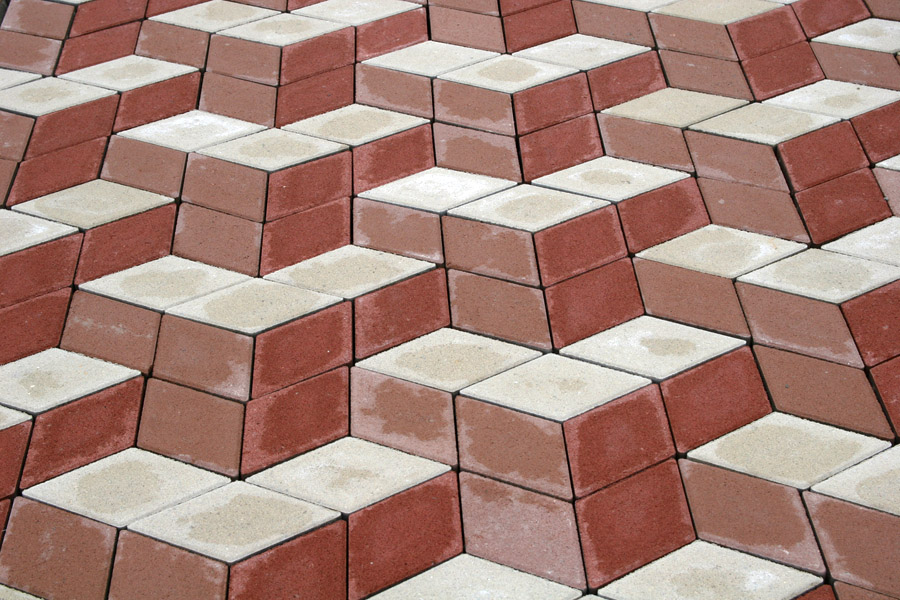
\includegraphics[width=.7\textwidth]{trotuar.jpg}
\end{center}

\end{frame}

\begin{frame}
Интересно, какие бывают плитки? Самая знакомая --- из прямоугольников:

\begin{center}
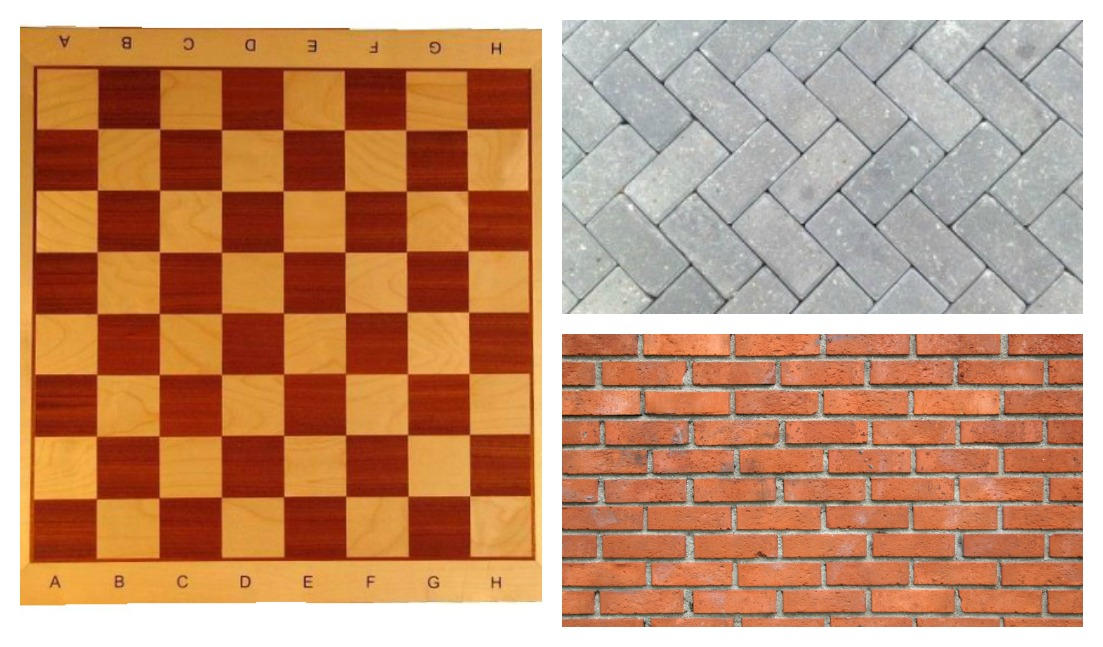
\includegraphics[width=\textwidth]{collage.jpg}
\end{center}

\end{frame}
\begin{frame}
Можно придумать еще одну плитку --- из правильных треугольников: 

\begin{center}
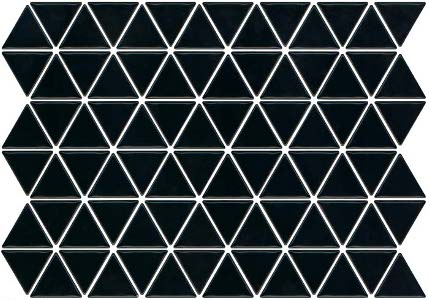
\includegraphics[width=.8\textwidth]{right_triangle.jpg}
\end{center}

\end{frame}

\begin{frame}
Забавно, что замостить можно плоскость любыми треугольниками. То, что это действительно замощение, следует из того, что сумма углов треугольника 180 градусов:

\begin{center}
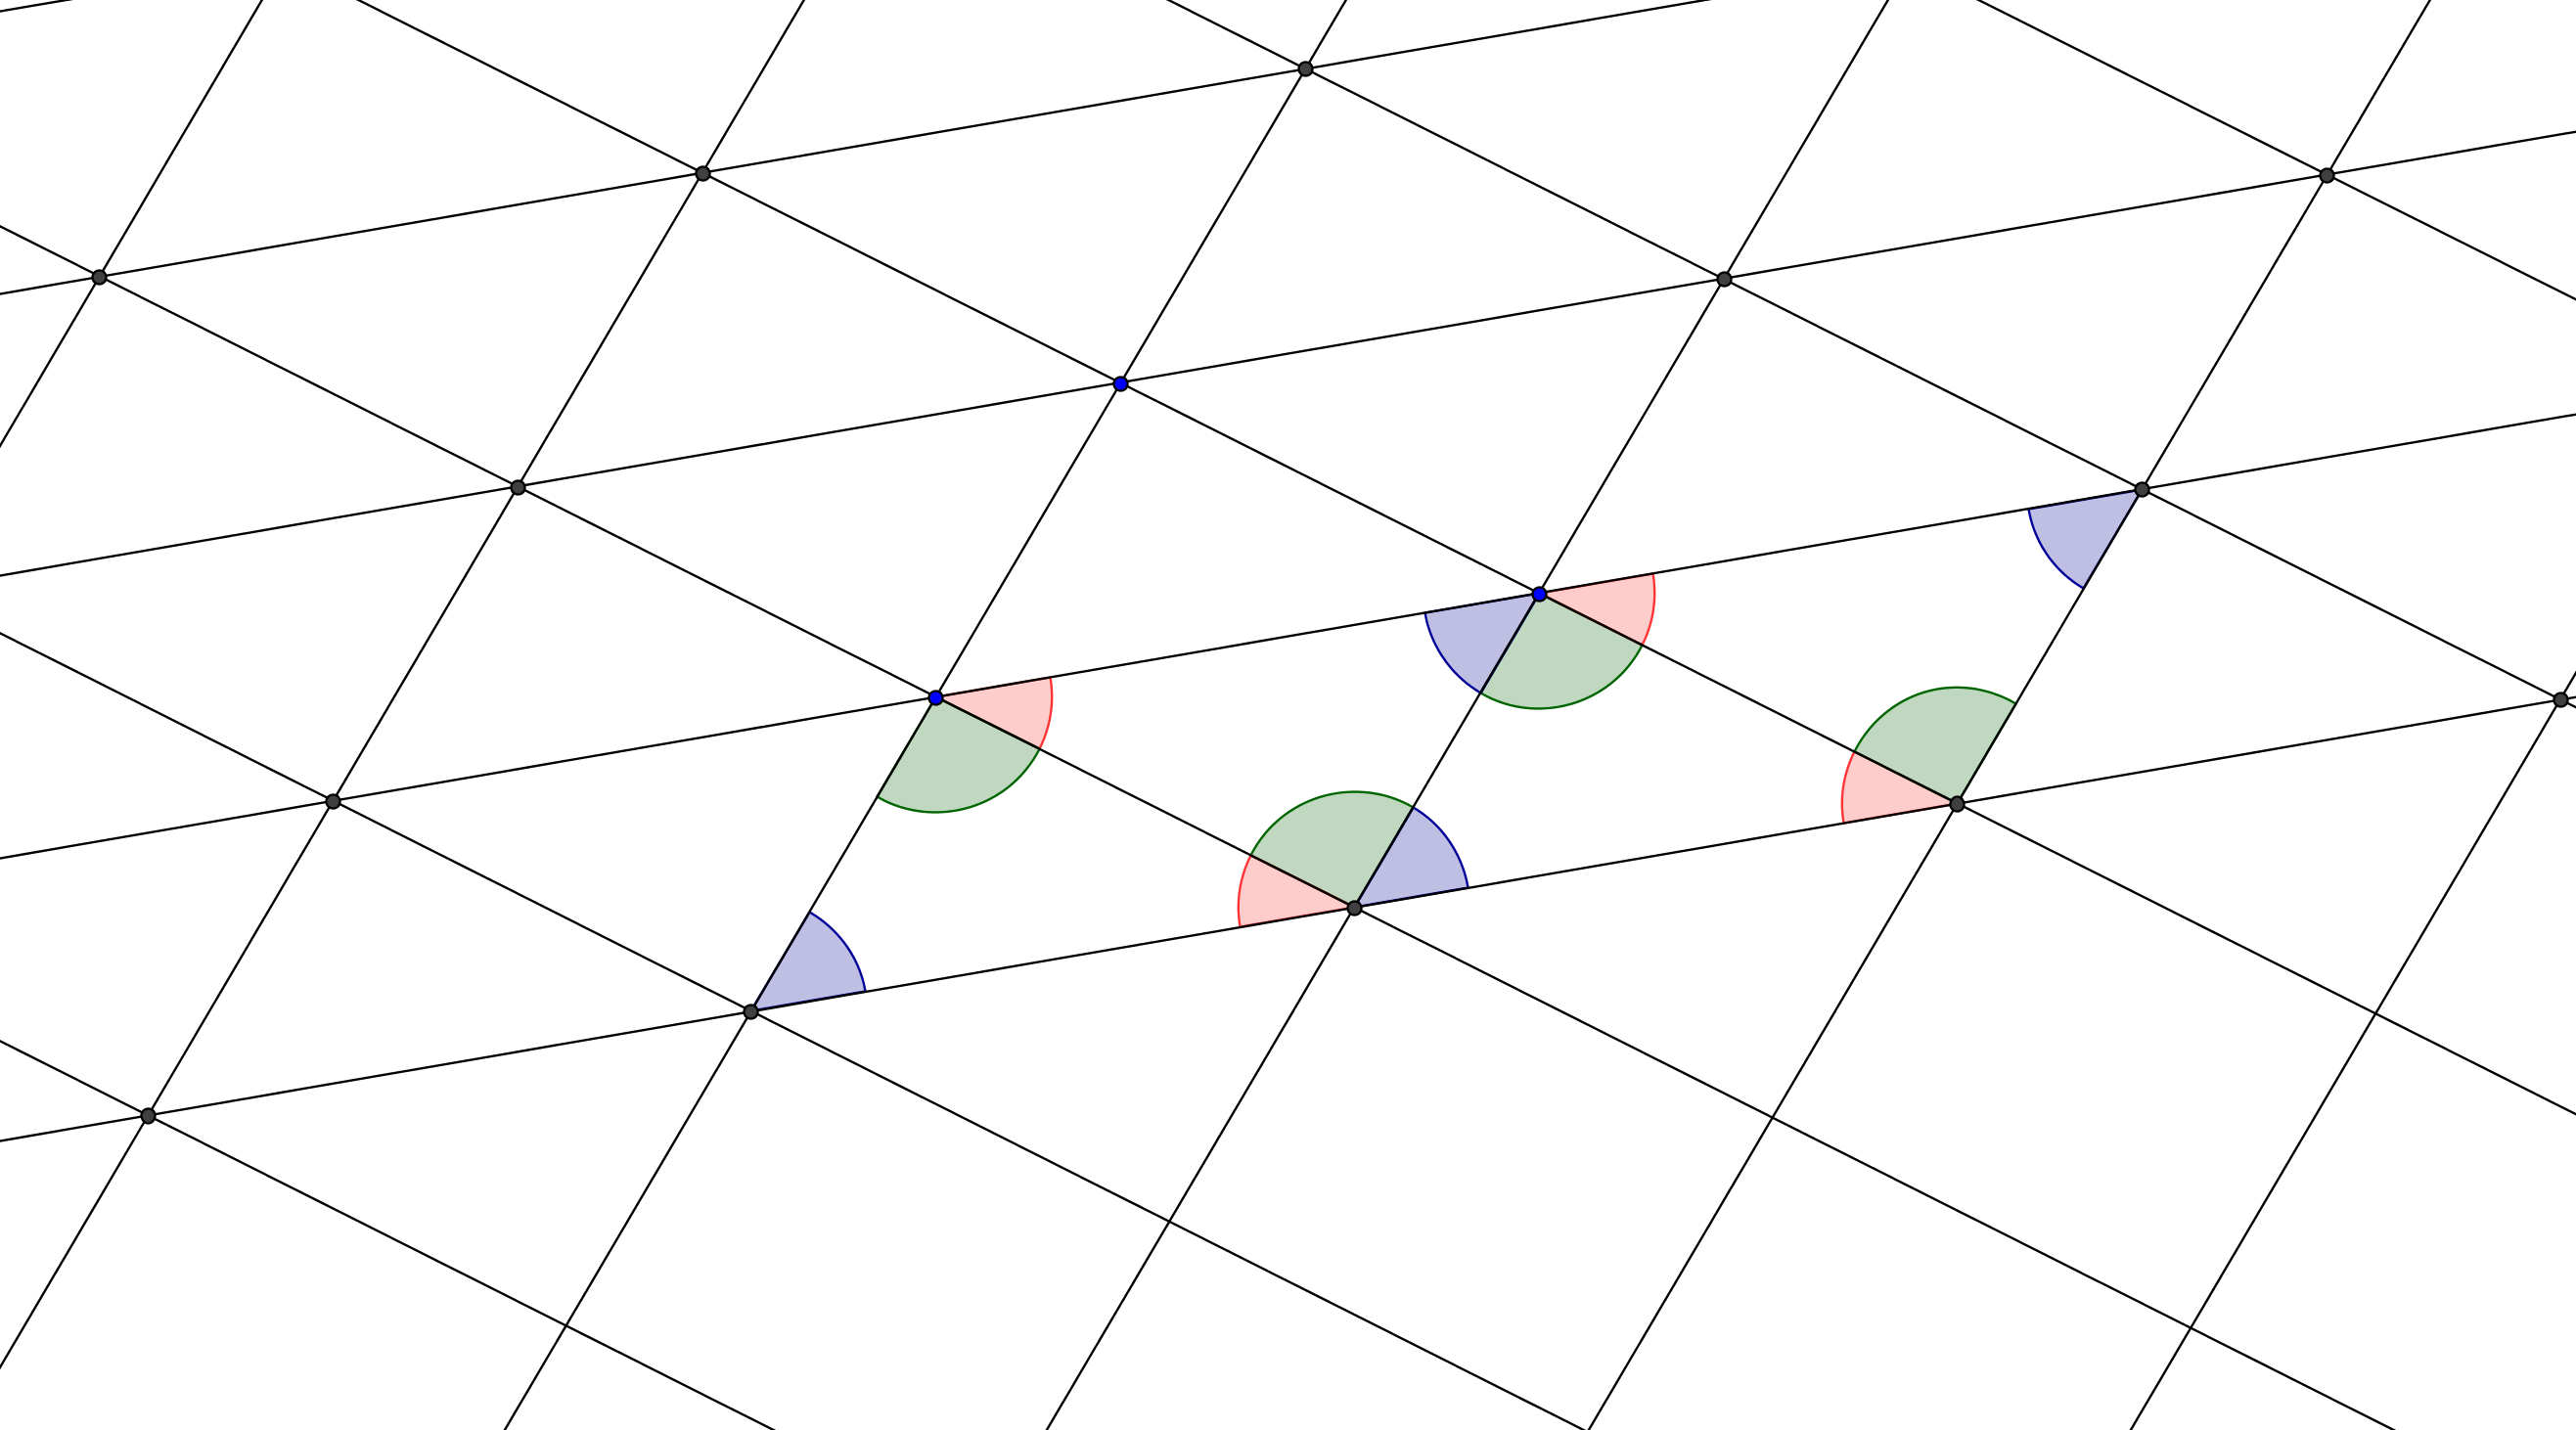
\includegraphics[width=\textwidth]{triangle.png}
\end{center}

\end{frame}


\begin{frame}

А какими четырехугольниками можно замостить плоскость?

\bigskip

\pause

Любыми!

\bigskip

\pause

\begin{theorem}
Плоскость можно замостить любым четырёхугольником.
\end{theorem}

\end{frame}

\begin{frame}

Идея замощения очень простая: будем укладывать четырехугольники диагоналями друг к другу:

\begin{center}
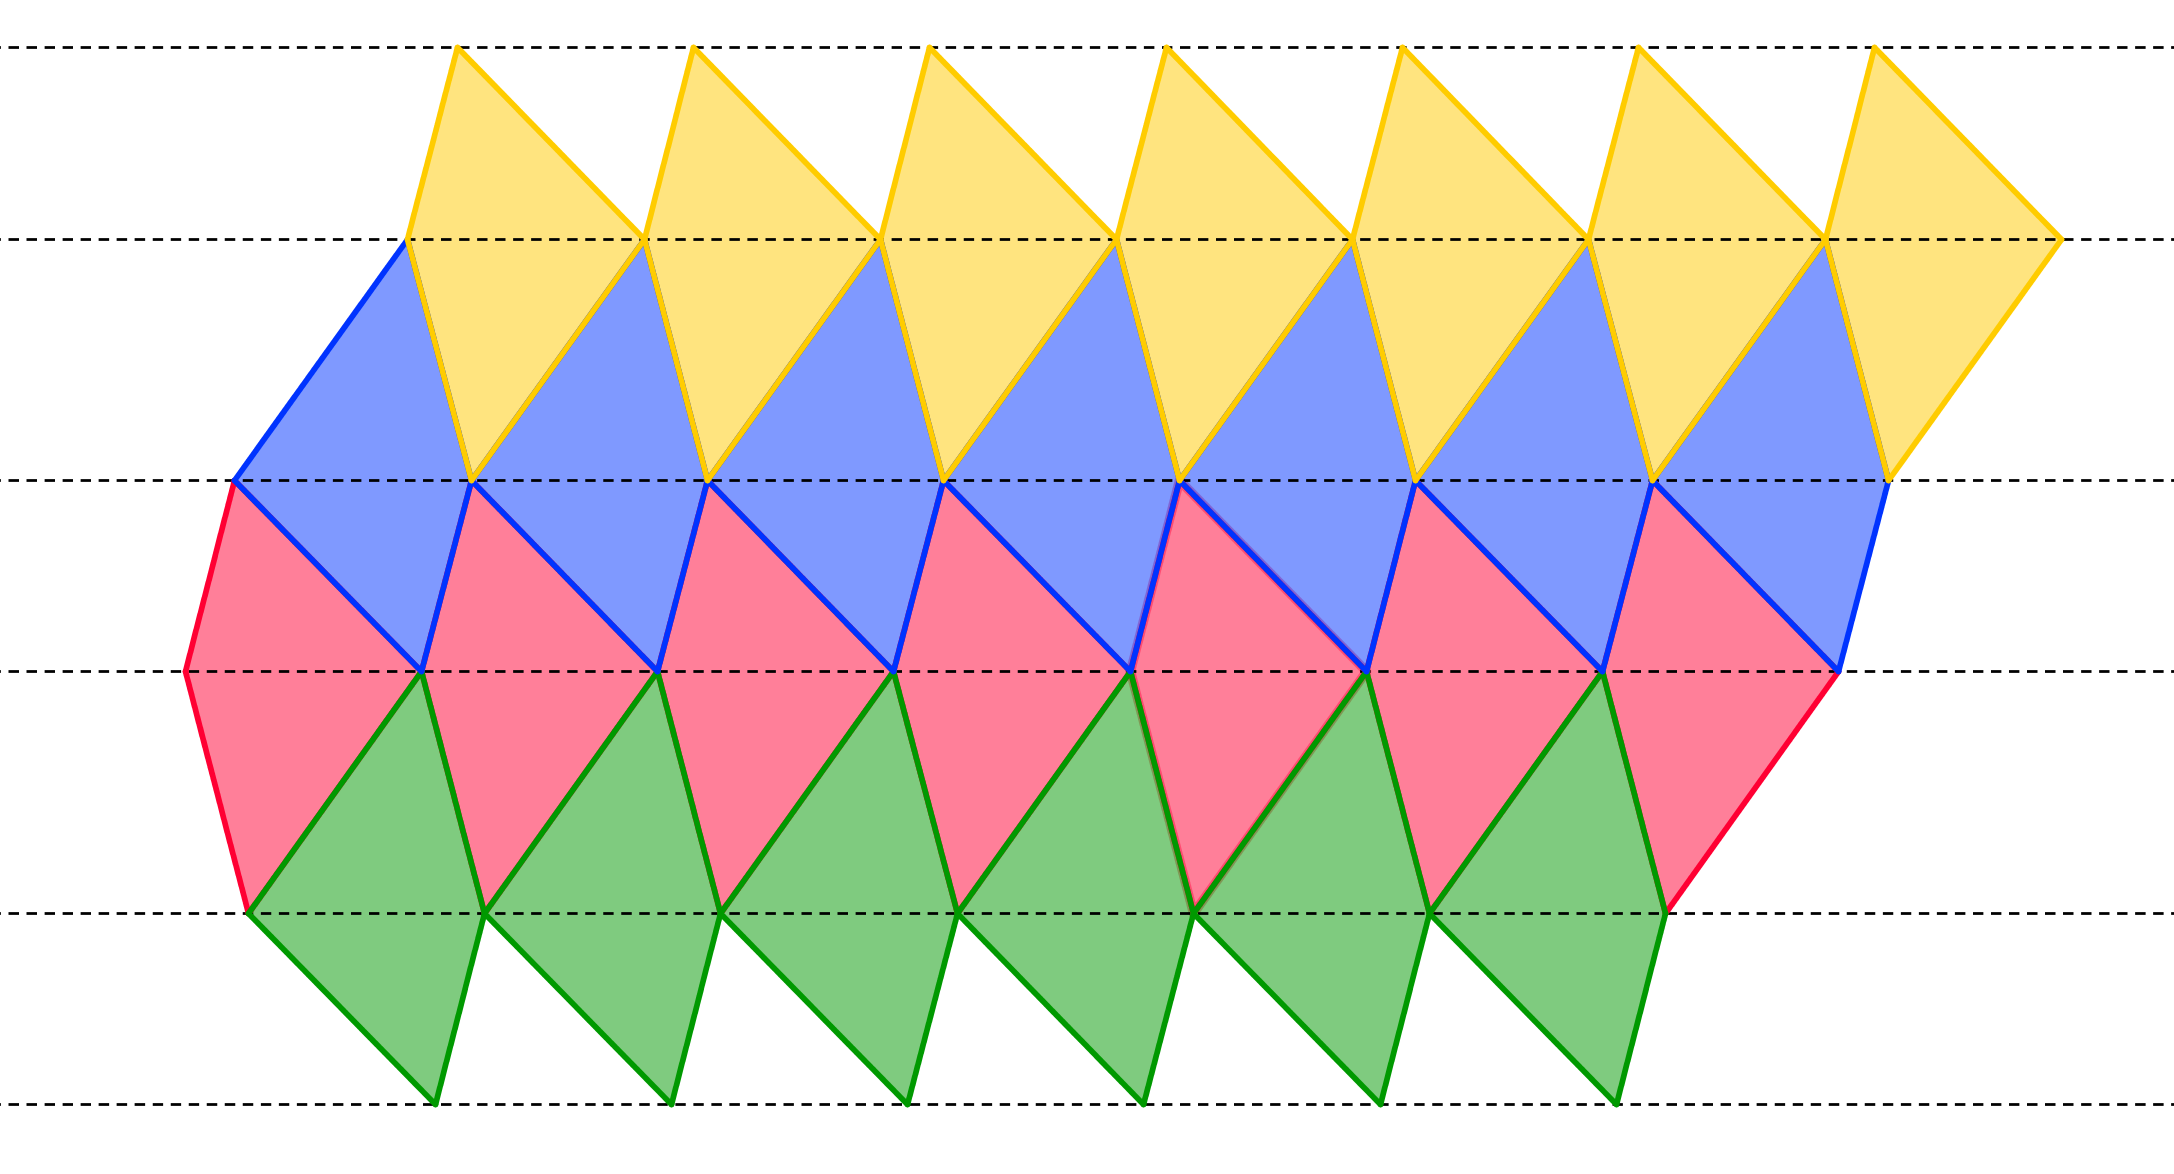
\includegraphics[width=\textwidth]{4-1.png}
\end{center}

\end{frame}


\begin{frame}
Кстати, то же построение подходит даже для невыпуклых четырехугольников:

\begin{center}
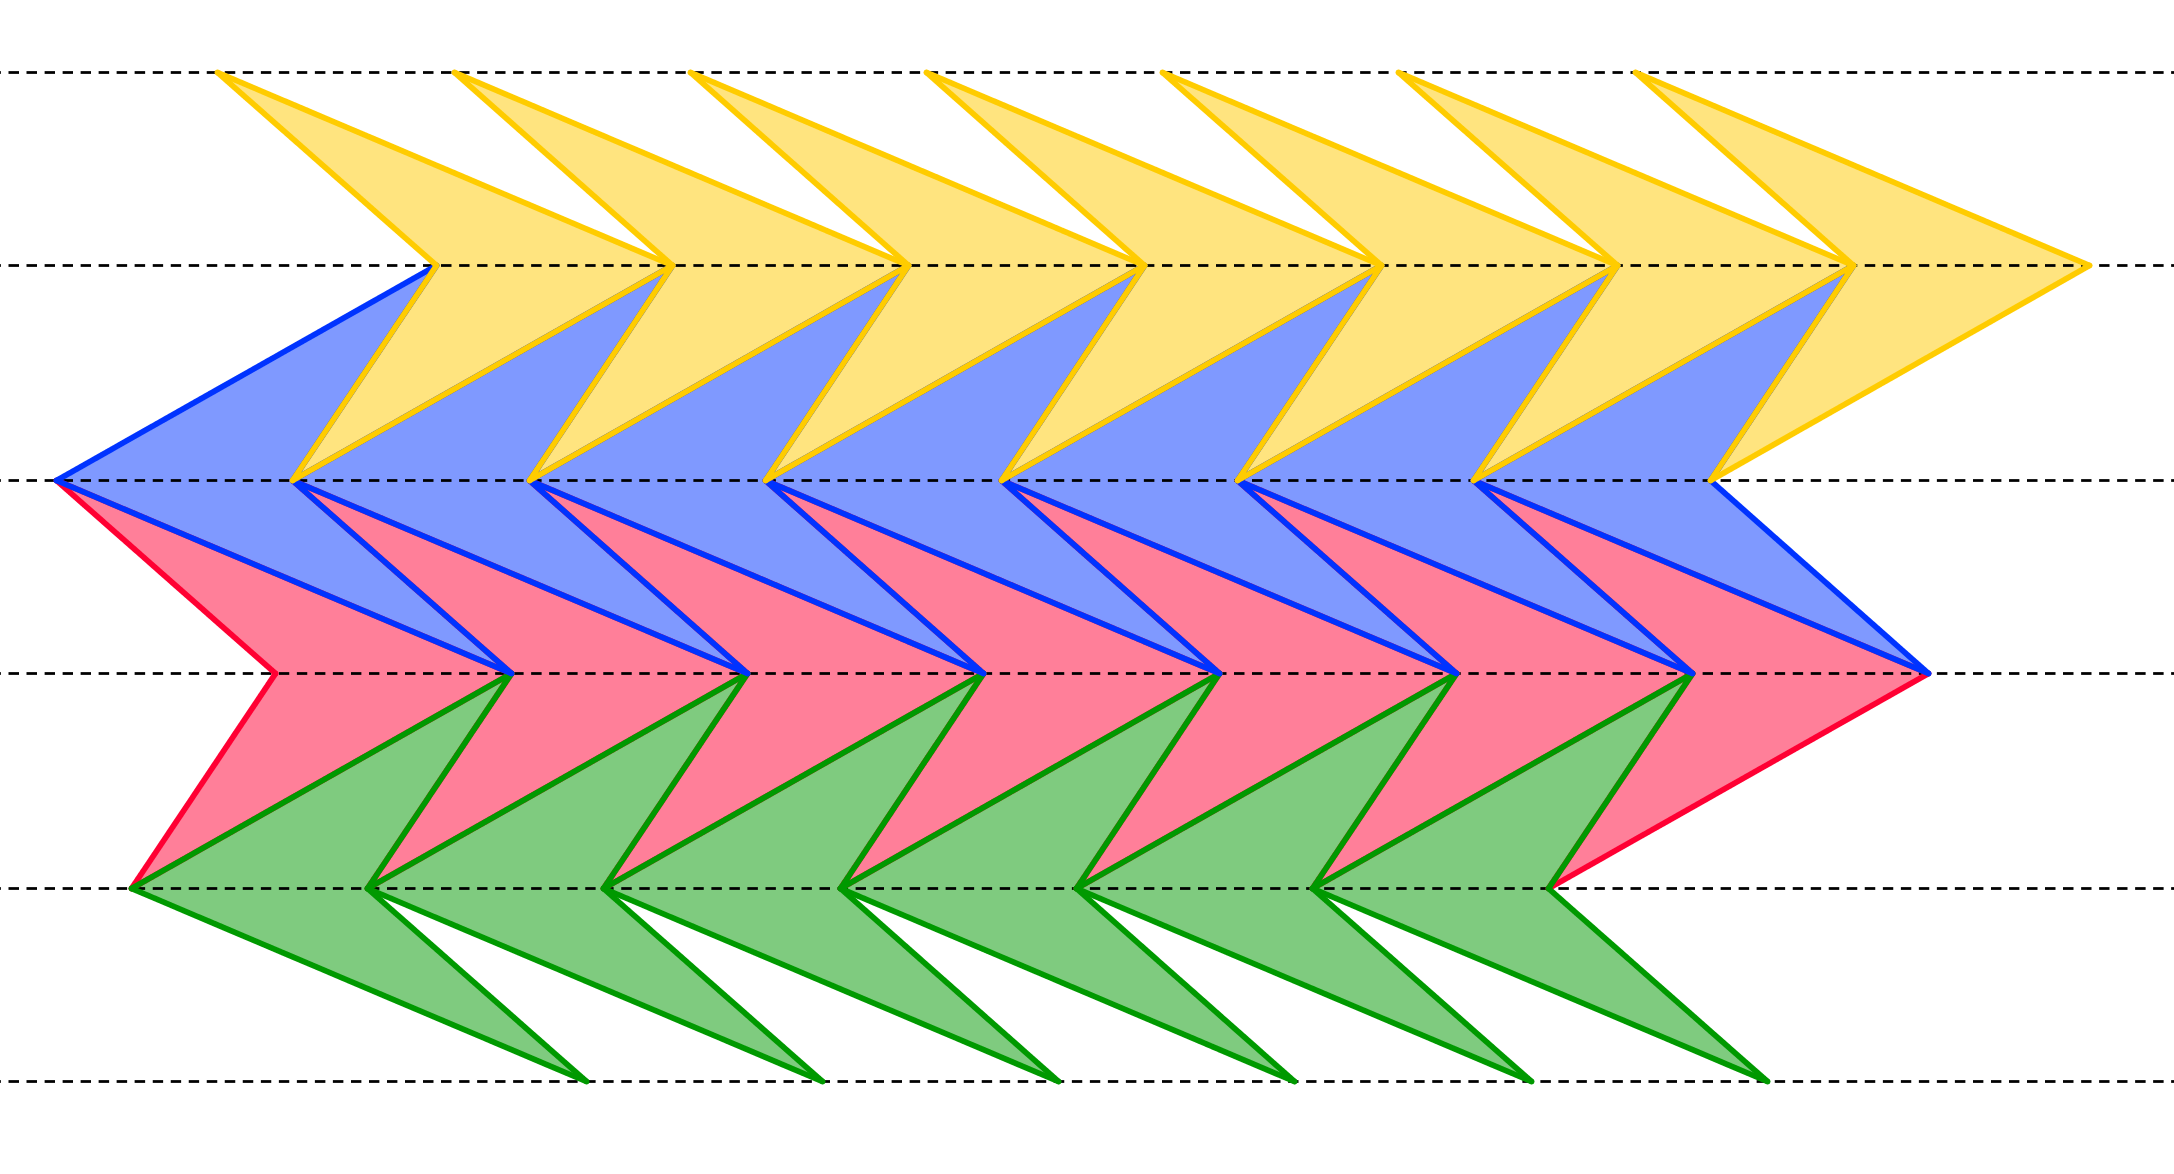
\includegraphics[width=\textwidth]{4-2.png}
\end{center}

\end{frame}

\begin{frame}
А как дела с пятиугольниками?

\medskip

\pause

Вот пример:

\begin{center}
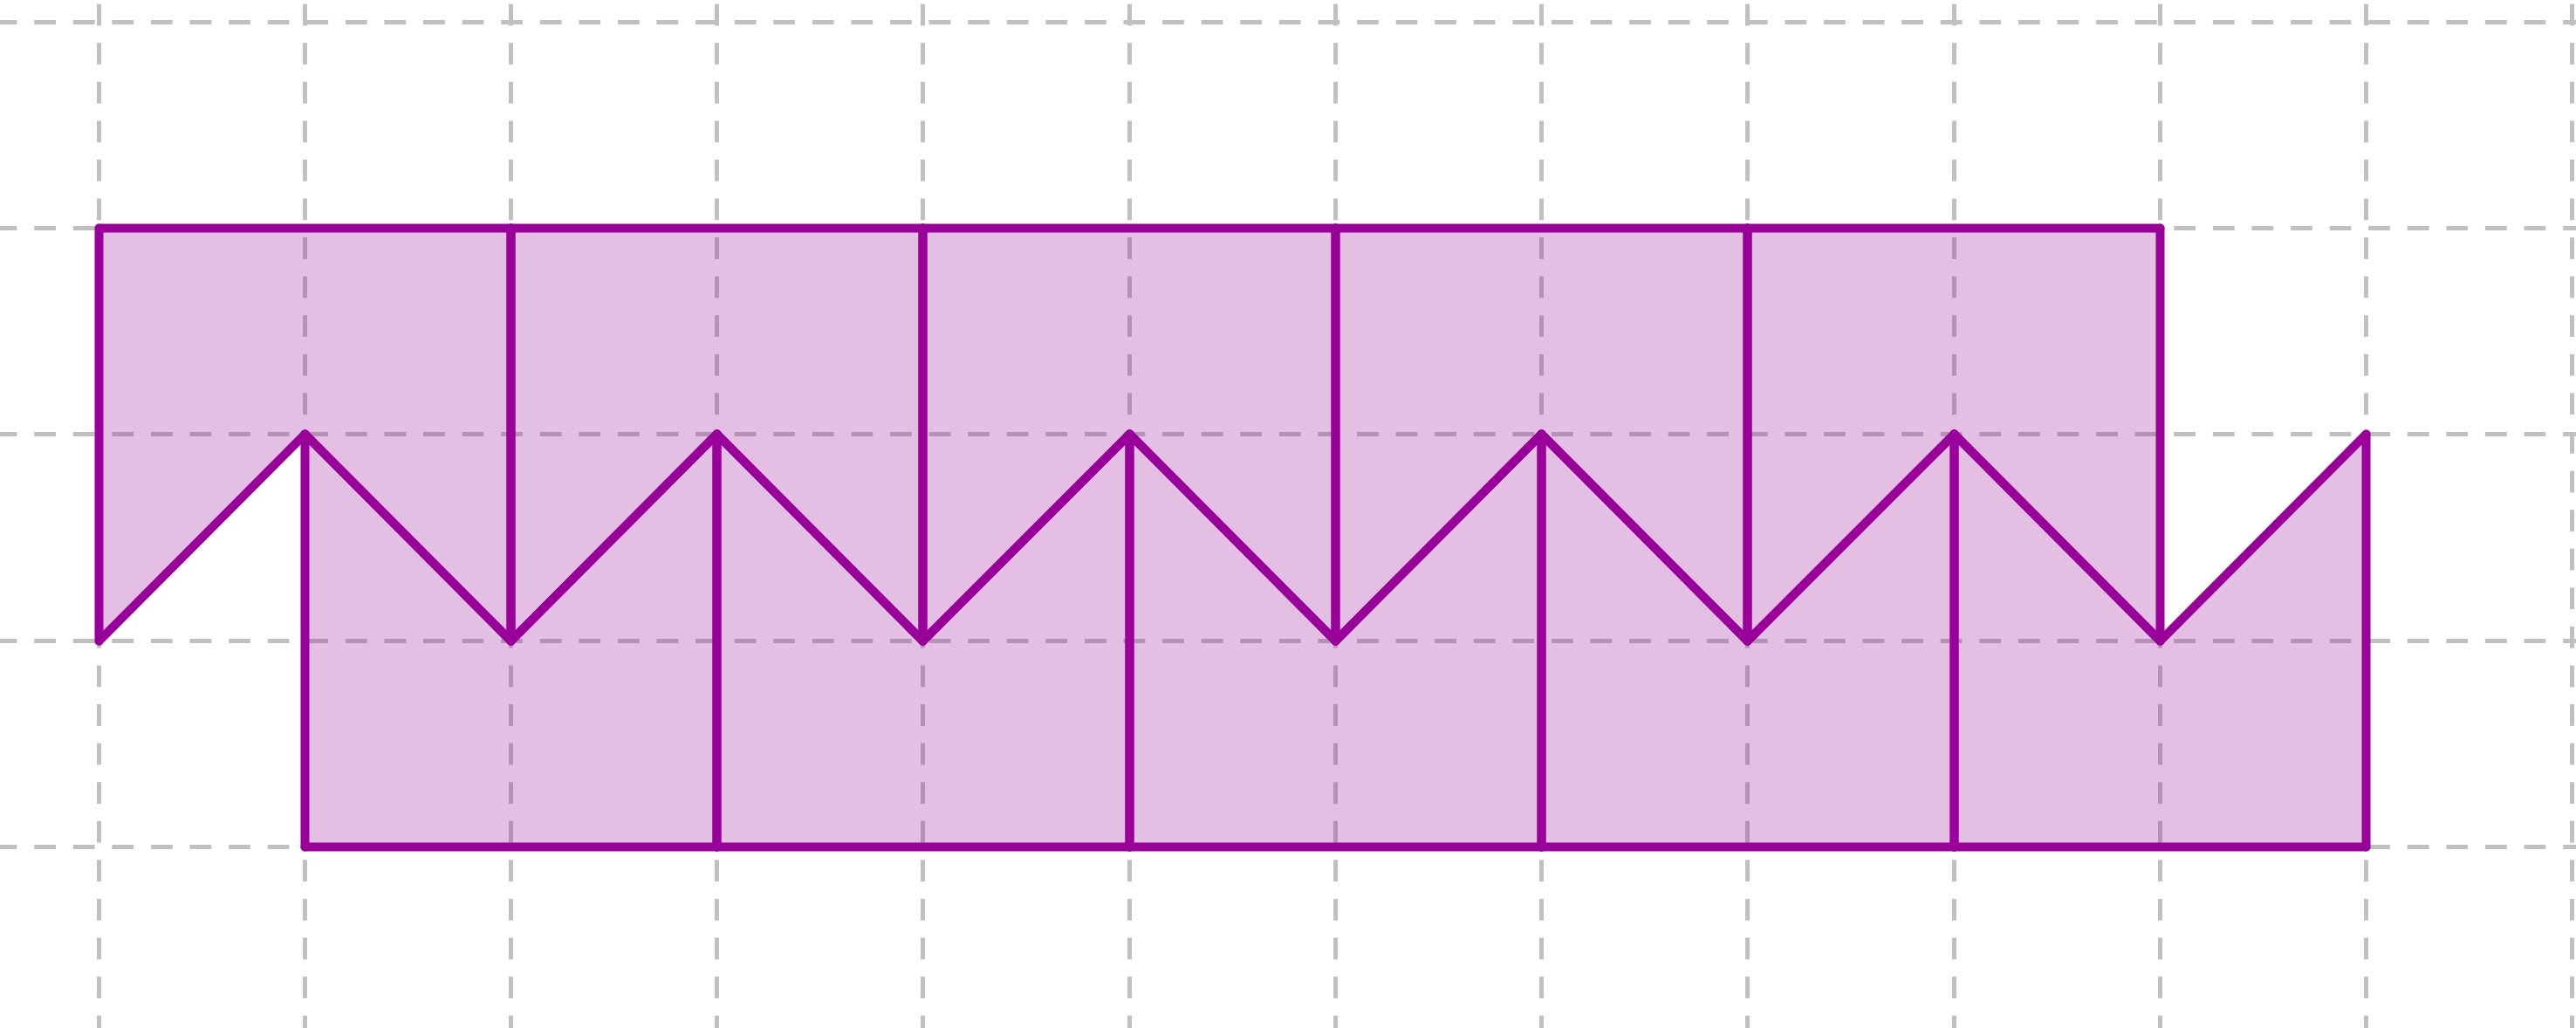
\includegraphics[width=\textwidth]{5-1.png}
\end{center}

\pause

\medskip

Он невыпуклый:(

\end{frame}


\begin{frame}

А есть замощения \emph{выпуклым} пятиугольником?

\medskip

\pause

Ок, для начала замостим плоскость шестиугольниками.

\pause


\begin{center}
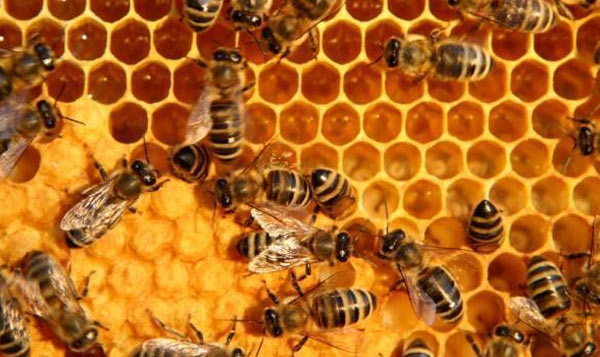
\includegraphics[width=.8\textwidth]{pcheli.jpg}
\end{center}

Это любая пчела может сделать! :)

\end{frame}

\begin{frame}

А теперь сделаем трюк!

Разрежем каждый шестиугольник на 3 одинаковых пятиугольника.

\vspace{-3ex}

\begin{center}
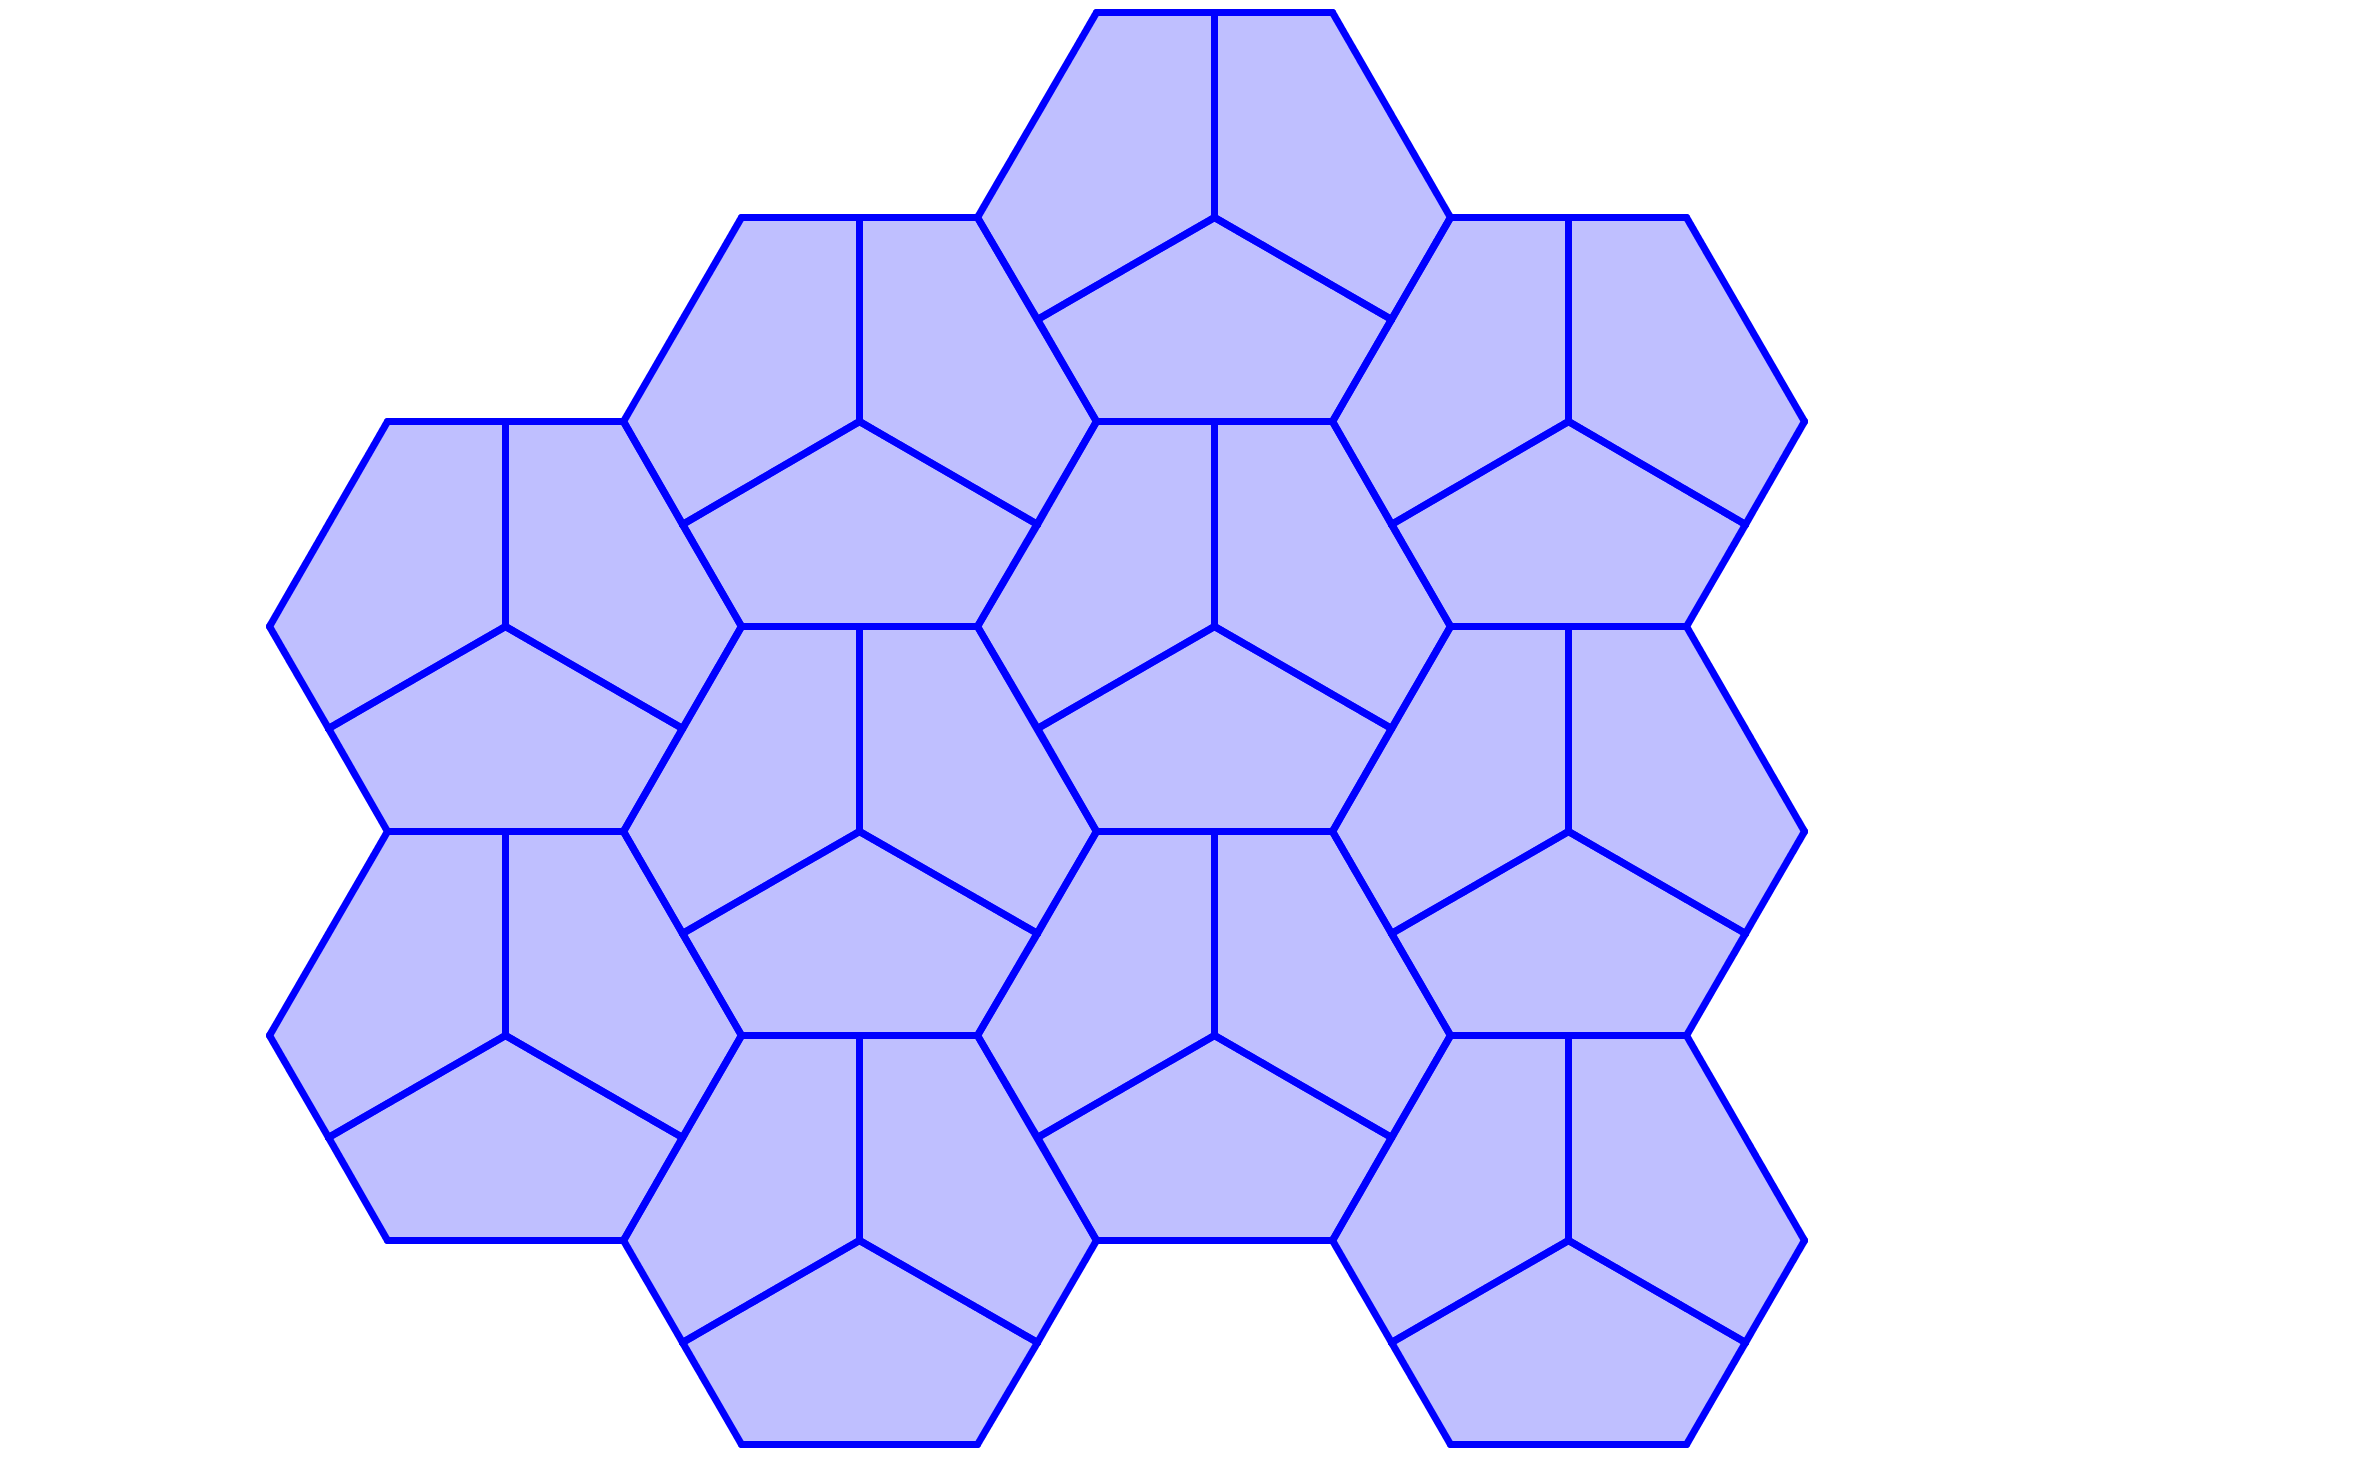
\includegraphics[width=\textwidth]{5-2.png}
\end{center}

\end{frame}


\begin{frame}
А какие еще бывают замощения пятиугольниками?

\pause

\medskip

Этот вопрос до сих пор открыт. Пока известно 15 замощений:

\begin{center}
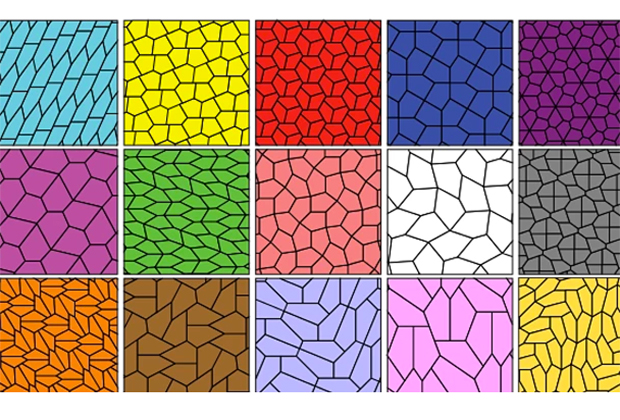
\includegraphics[width=\textwidth]{5-all.jpg}
\end{center}

\end{frame}

\begin{frame}

Замощение таким пятиугольником было открыто совсем недавно, в июле 2015 года:

\begin{center}
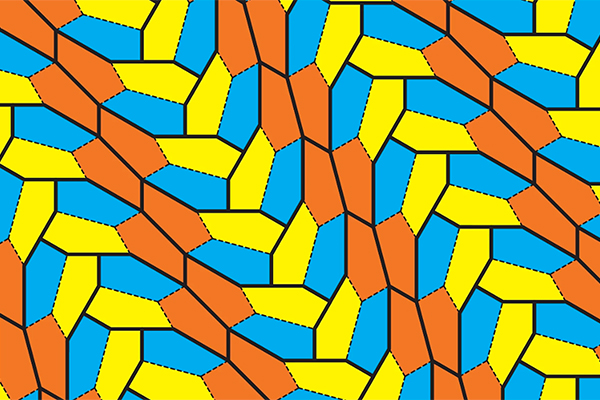
\includegraphics[width=\textwidth]{5-new.jpg}
\end{center}

\end{frame}

\begin{frame}
Замощение устроено довольно хитроумно:

\begin{center}
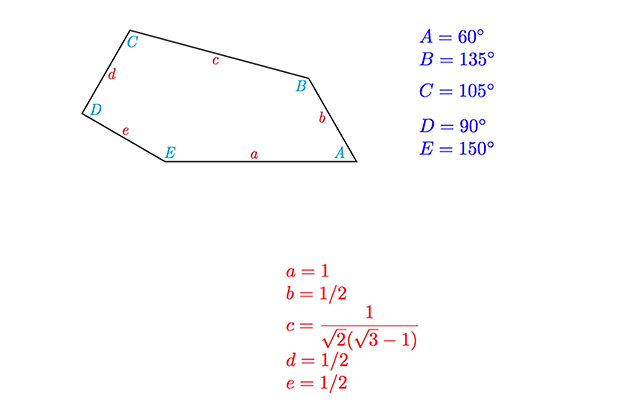
\includegraphics[width=\textwidth]{5-new-size.jpg}
\end{center}

\end{frame}


\begin{frame}
Понять, почему же это действительно замощение, можно из такой странной картинки:

\vspace{-2ex}

\begin{center}
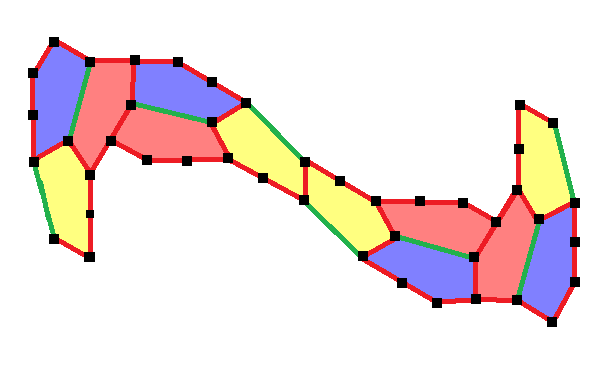
\includegraphics[width=\textwidth]{lattice.png}
\end{center}

\vspace{-6ex}

\pause

Обратите внимание, что эта фигурка после параллельного сдвига идеально <<пристыковывается>> сама к себе.

\end{frame}

\begin{frame}
А эти 4 замощения открыта домохозяйка Марджори Райс, изучив статью Мартина Гарднера в журнале Scientific American\footnote{Журнал, кстати, выписывал сын.}:

\begin{center}
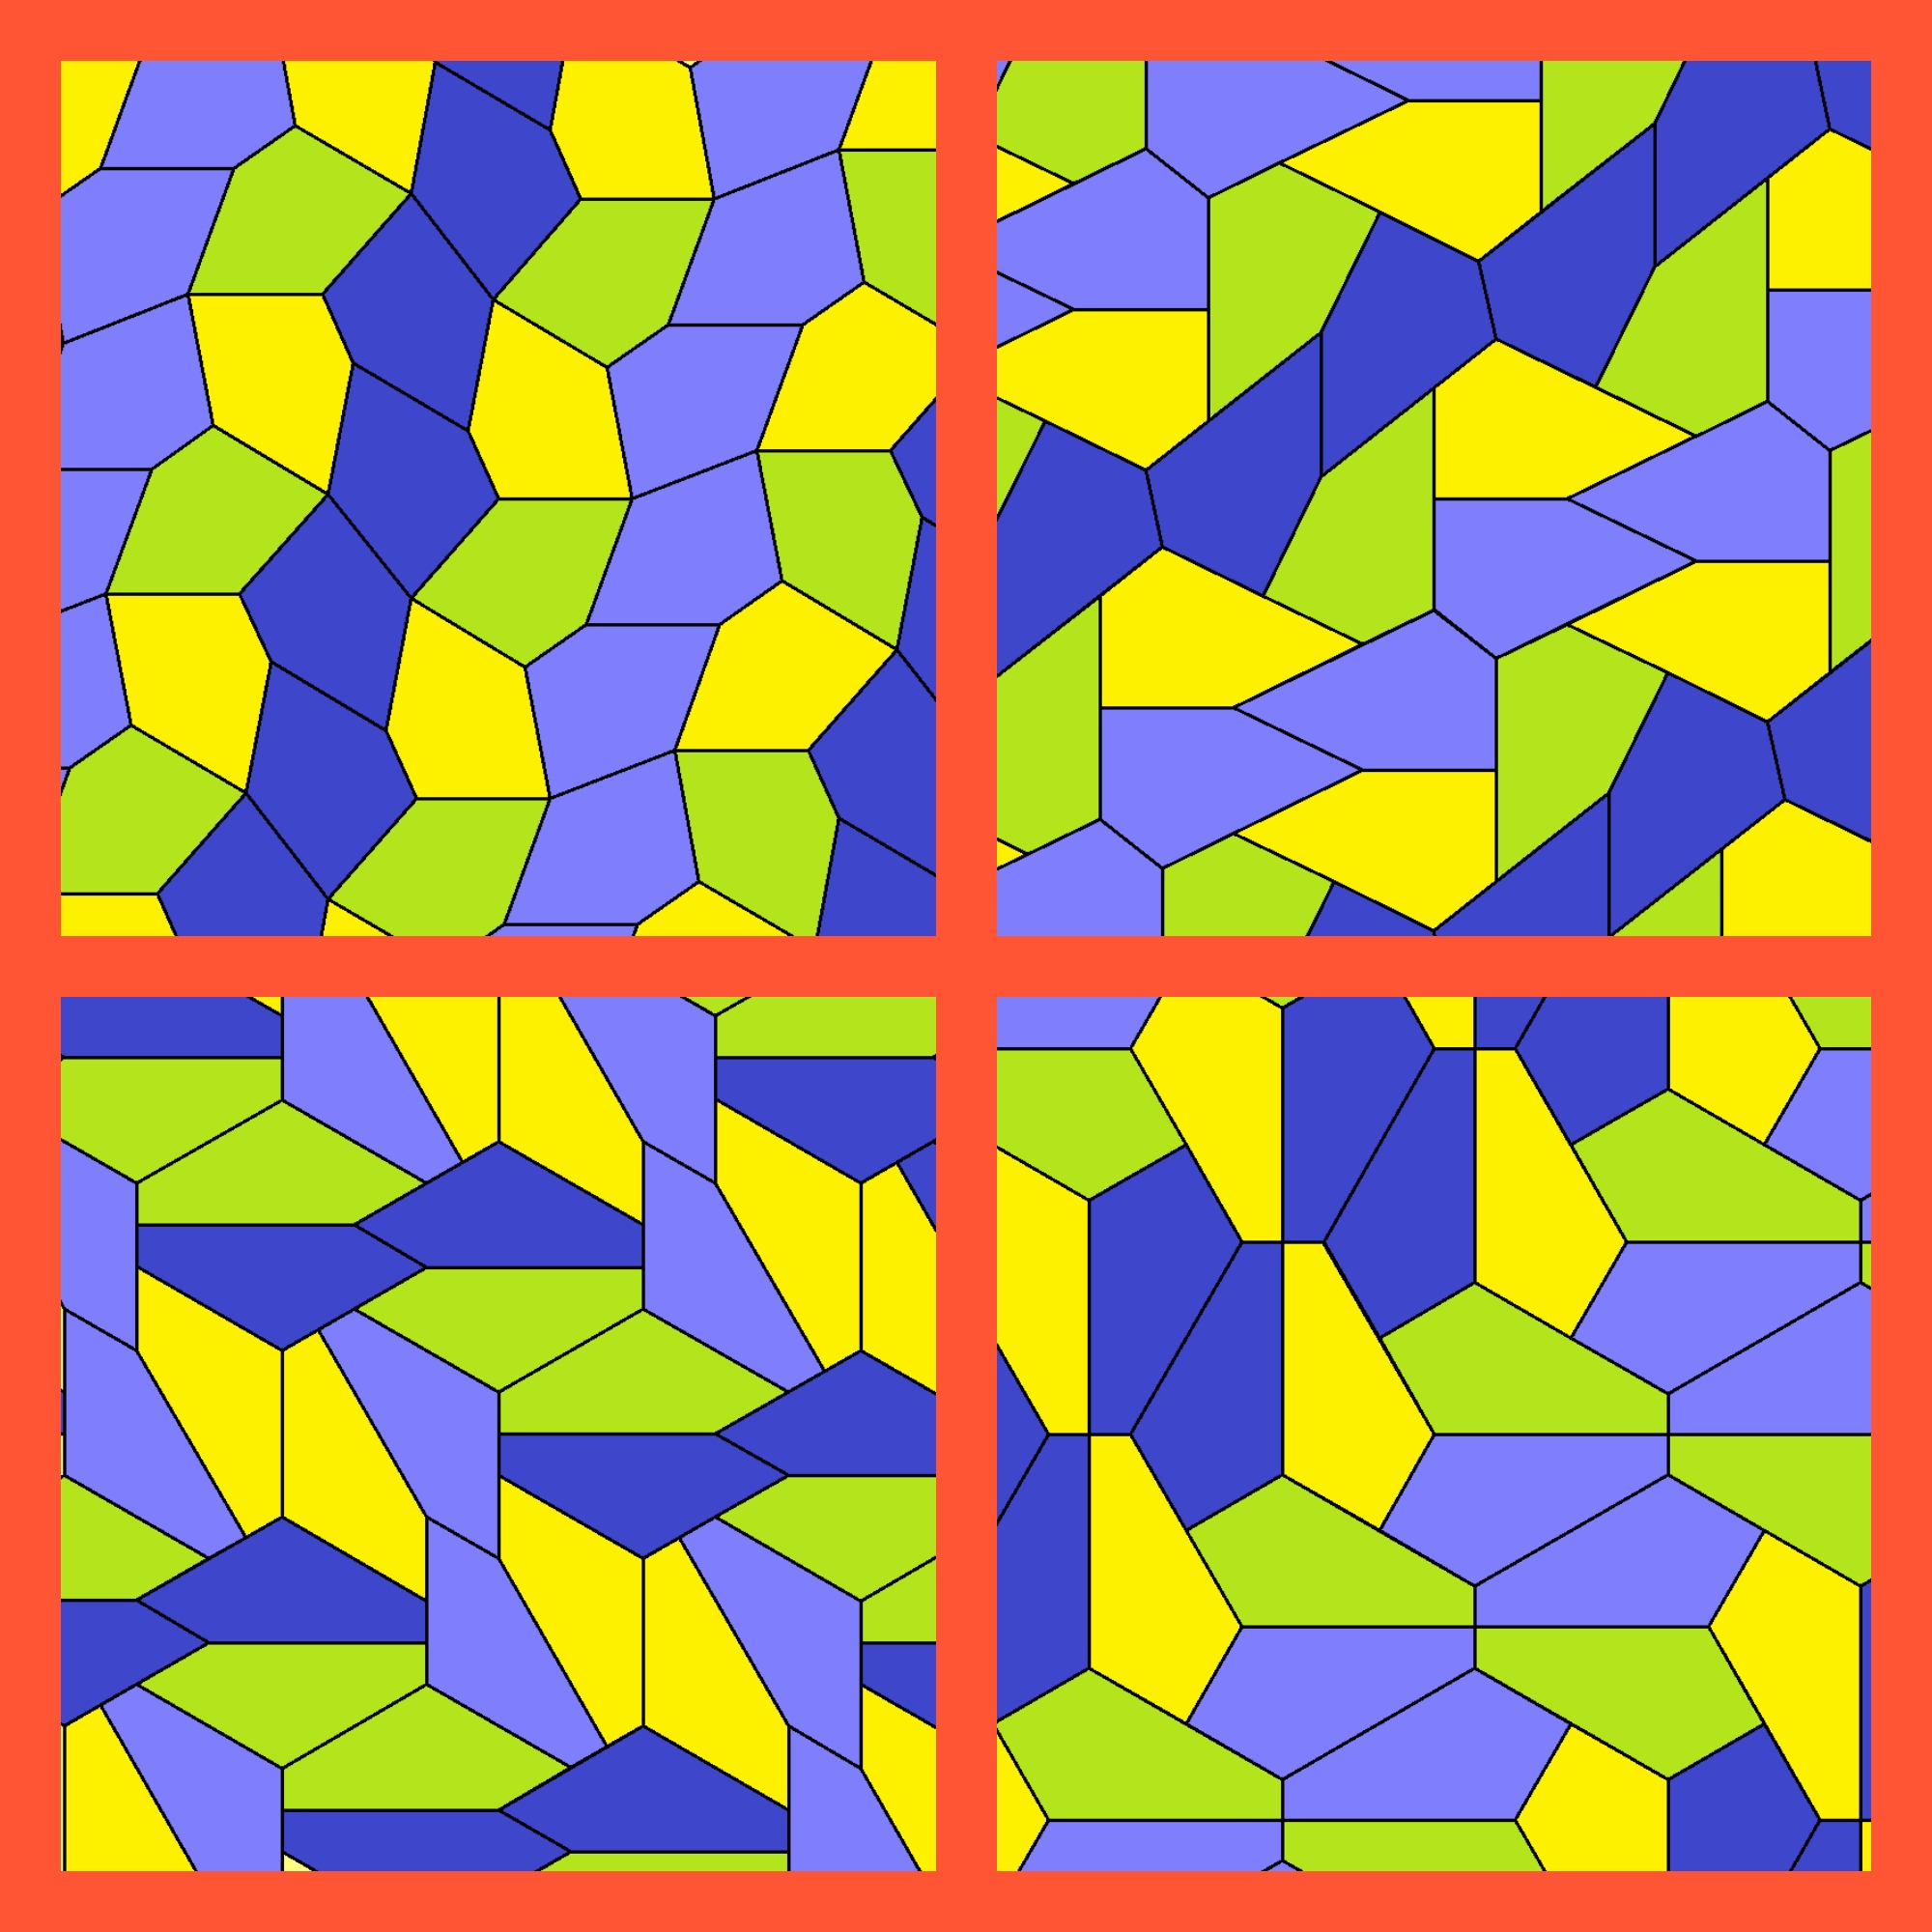
\includegraphics[width=.6\textwidth]{collage_rice.jpg}
\end{center}

\end{frame}

\begin{frame}

Ок, пятиугольники --- это очень интересно. 

\medskip

А что, например, с 15-угольниками?

\medskip

\pause

\begin{theorem}
Никаким \emph{выпуклым} $n$-угольником с $n \geqslant 6$ нельзя замостить плоскость.
\end{theorem}

\medskip

\pause

\begin{itemize}

\item А если $n$-угольник \emph{невыпуклый}?\pause

\item А можно замостить плоскость \emph{различными выпуклыми} $n$-угольниками?
\end{itemize}

\end{frame}


\begin{frame}
Ок, многоугольники --- это очень интересно, но это все на плоскости. 

\pause

\bigskip

В пространстве есть замощения?
\end{frame}


\begin{frame}

Есть! Например, кубиками точно можно замостить :)


\begin{center}
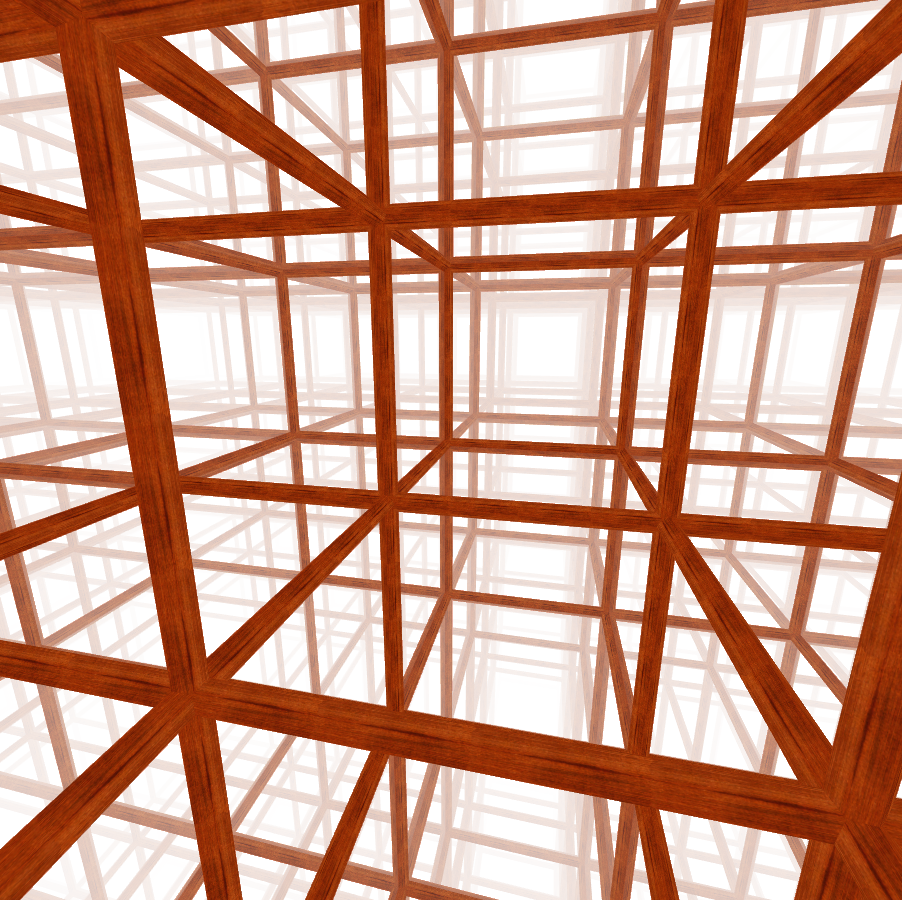
\includegraphics[width=.6\textwidth]{Cubic_honeycomb.png}
\end{center}

\end{frame}

\begin{frame}

А призмами можно?

\pause

Да!

\medskip

\begin{center}
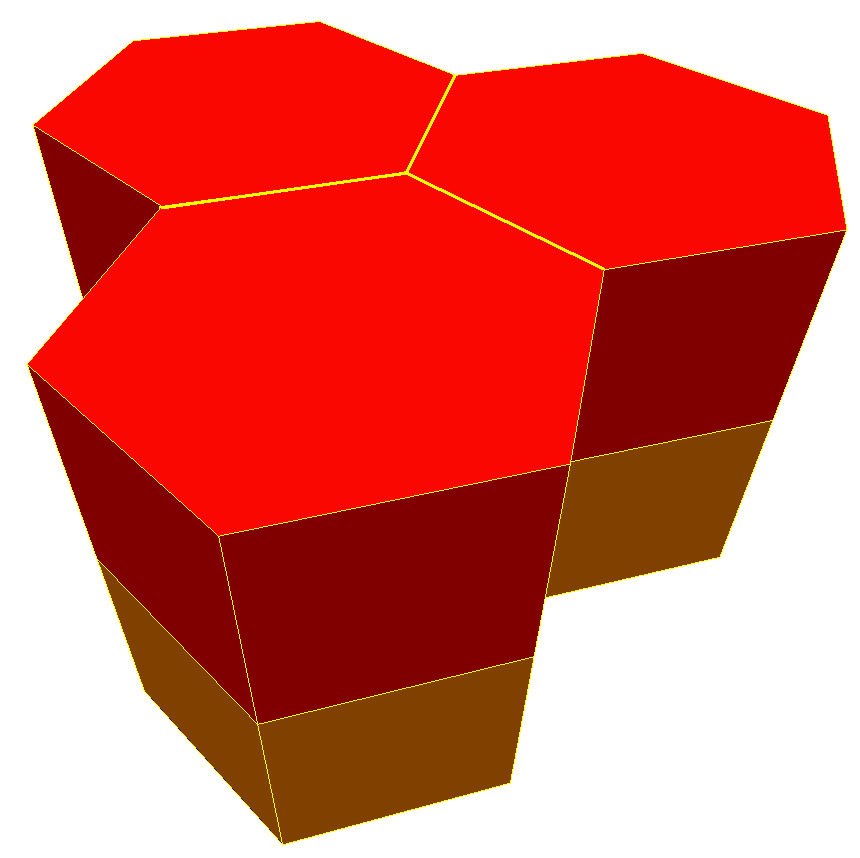
\includegraphics[width=.6\textwidth]{Hexagonal_prismatic_honeycomb.png}
\end{center}

\end{frame}

\begin{frame}

Можно даже \emph{гексаромбическим додекаэдром}!

\begin{center}
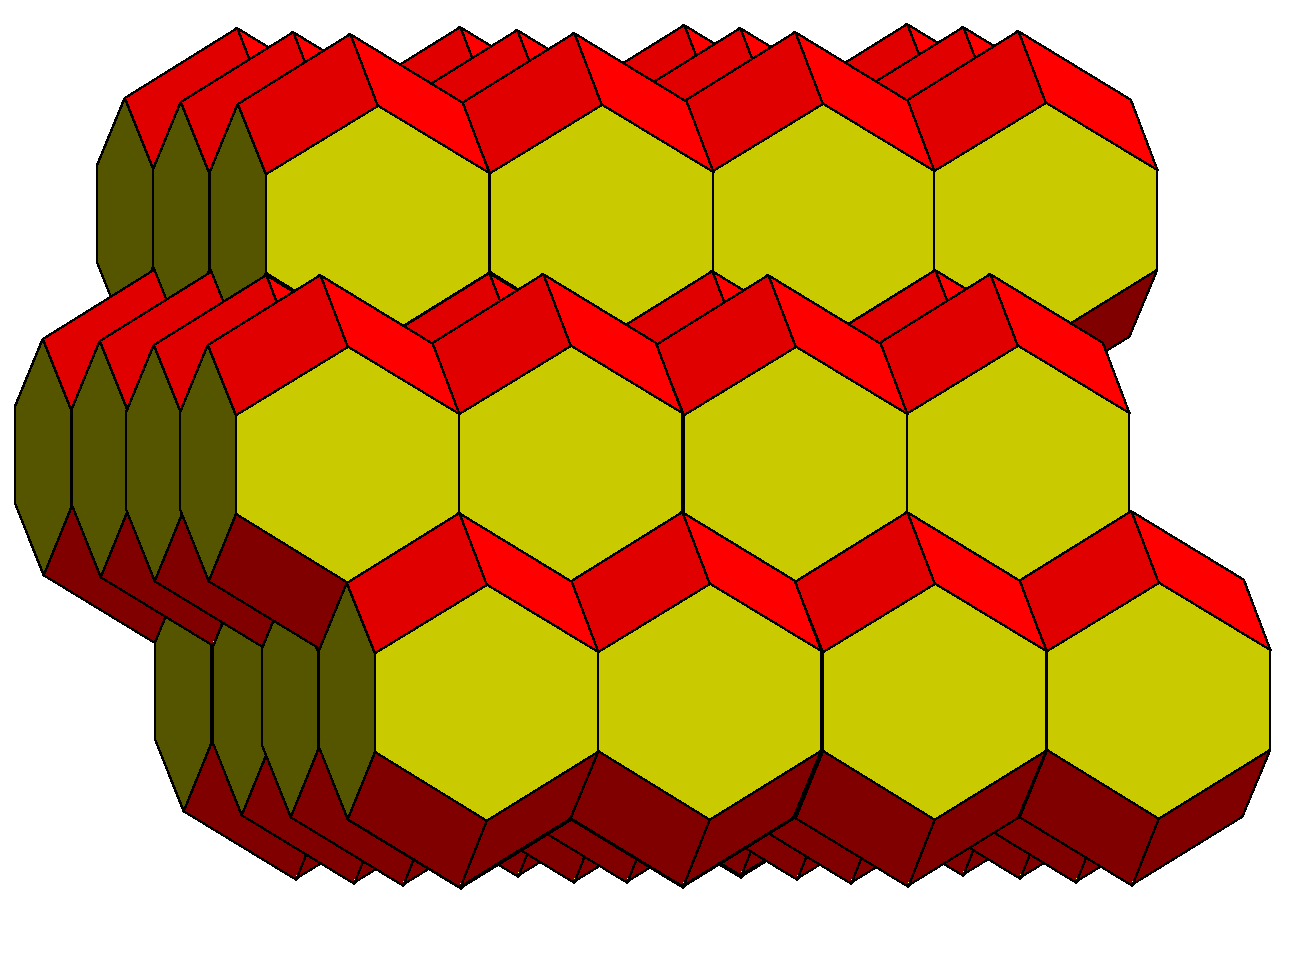
\includegraphics[width=\textwidth]{Rhombo-hexagonal_dodecahedron_tessellation.png}
\end{center}


\vspace{-11ex}


\includegraphics[width=.1\textwidth]{meme.png}
\end{frame}


\begin{frame}
А вот ещё одно замощение пространства --- усечённым октаэдром:

\vspace{-2ex}


\begin{center}
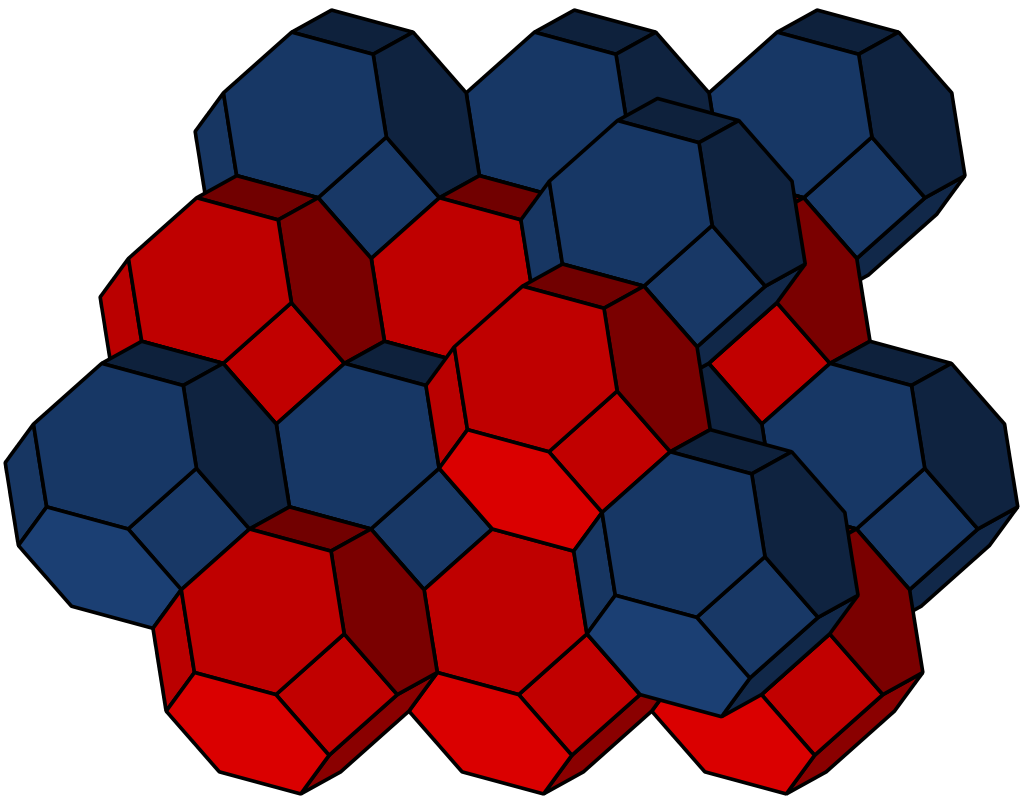
\includegraphics[width=.7\textwidth]{Bitruncated_Cubic_Honeycomb.png}
\end{center}

\pause

Оно кажется очень сложным, но на самом деле легко получается из замощения пространства кубиками.


\end{frame}

\begin{frame}
Для начала нужно разобраться, как же выглядит усечённый октаэдр:

\vspace{-3ex}

\begin{center}
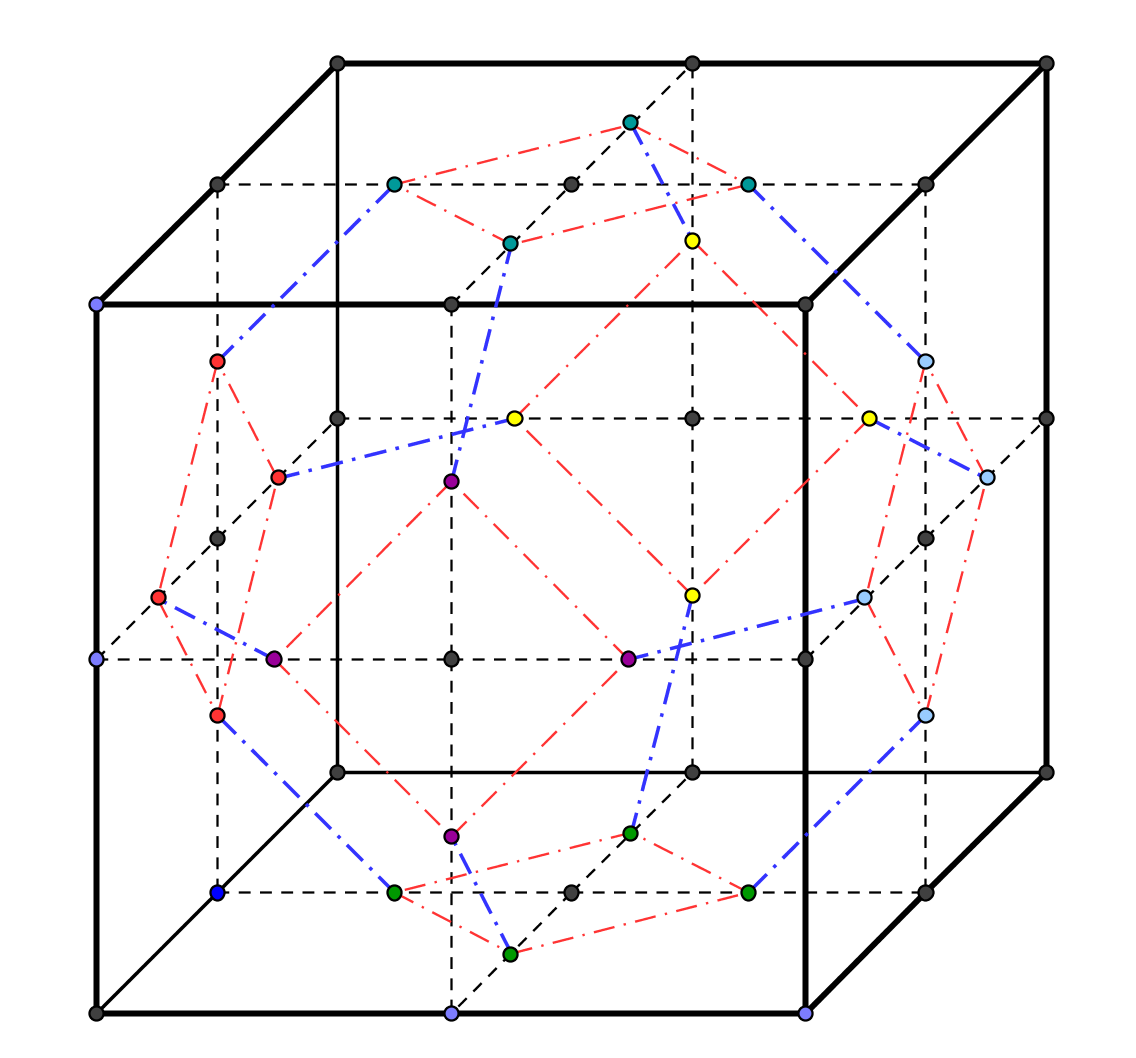
\includegraphics[width=.8\textwidth]{octahedron.png}
\end{center}

\end{frame}


\begin{frame}

Рассмотрим центры кубиков $A_i$, замощающих пространство. 

\bigskip

Понятно, что эти центры --- вершины кубиков $B_j$, тоже замощающих пространство.

\end{frame}


\begin{frame}

Синие усечённые октаэдры вписаны в кубики $A_i$, а красные  --- в $B_j$.

\begin{center}
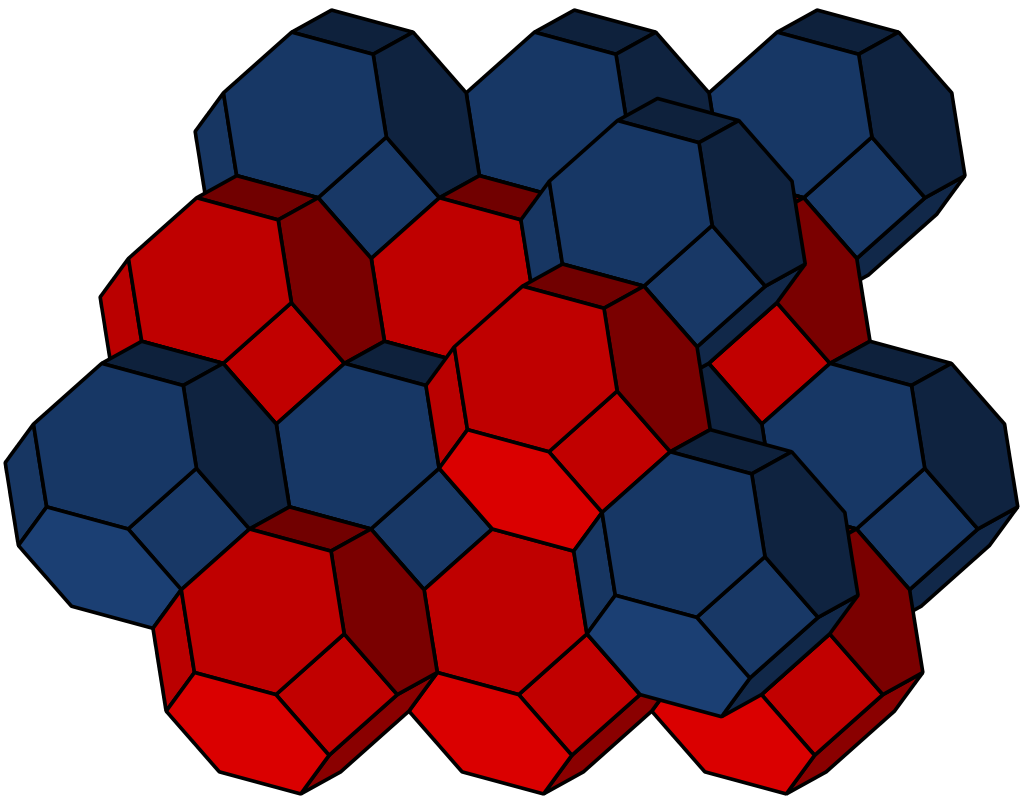
\includegraphics[width=.8\textwidth]{Bitruncated_Cubic_Honeycomb.png}
\end{center}

\end{frame}


\begin{frame}

Какими многогранниками можно замостить пространство?

\pause

\bigskip

Этот вопрос до сих пор не решён.

\bigskip

Классифицированы только замощения правильными и полуправильными многогранниками.

\pause

\begin{theorem}
Среди правильных многогранников (правильный тетраэдр, куб, октаэдр, додекаэдр, икосаэдр) пространство можно замостить только кубом.
\end{theorem}


\pause

\begin{itemize}
\item Докажите, что пространство нельзя замостить правильным тетраэдром.
\end{itemize}

\end{frame}


\begin{frame}
Мы поговорили о замощениях на плоскости и в пространстве.

\pause

А теперь --- замощение плоскости Лобачевского треугольниками!

\begin{center}
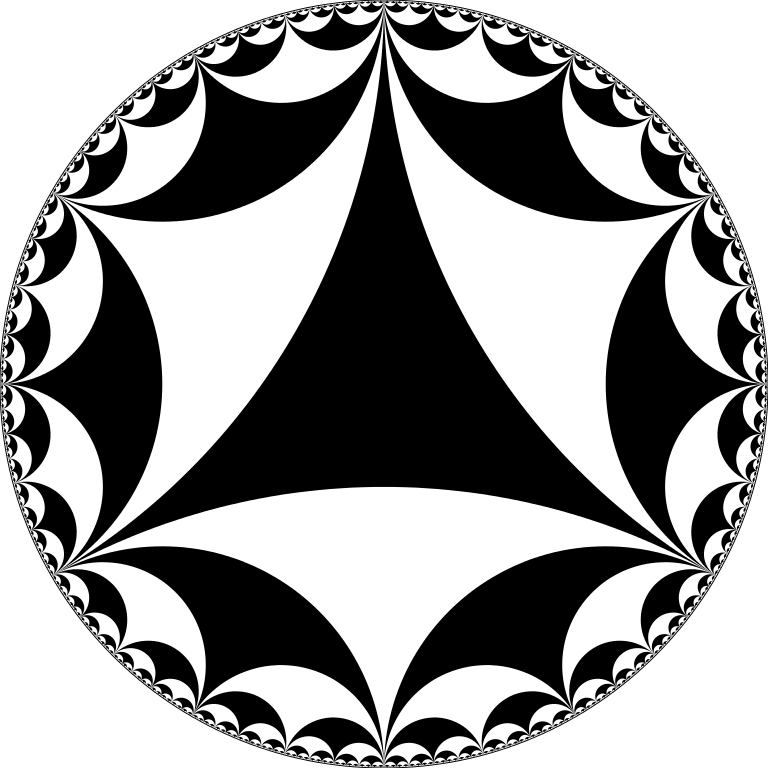
\includegraphics[width=.65\textwidth]{hyperbolic.png}
\end{center}

\end{frame}


%А что с пирамидой? Например, с самой простой -- с правильным тетраэдром?
%
%Правильным тетраэдром нельза замостить пространство.
%
%Почему?
%
%Пусть можно. Тогда вокруг ребра должно быть несколько тетраэдров:
%
%Разрежем замощение перпендикулярно ребру:
%
%Какими могут быть заштрихованные углы?
%
%А чему равны эти углы у тетраэдра?



\end{document}


}
